\documentclass[a4paper]{article}
\usepackage{geometry}
\usepackage{algpseudocode}
\usepackage{algorithm}
\usepackage{algorithmicx}
\usepackage{graphicx}
\usepackage{amsmath}
\usepackage{booktabs}
\usepackage{dsfont}
\usepackage{paralist}
\usepackage{epstopdf}
\usepackage{tabularx}
\usepackage{longtable}
\usepackage{multirow}
\usepackage{multicol}
\usepackage[hidelinks]{hyperref}
\usepackage{fancyvrb}
\usepackage{float}
\usepackage{paralist}
\usepackage[svgname]{xcolor}
\usepackage{enumerate}
\usepackage{array}
\usepackage{times}
\usepackage{url}
\usepackage{fancyhdr}
\usepackage{comment}
\usepackage{environ}
\usepackage{times}
\usepackage{textcomp}
\usepackage{caption}
\usepackage[square,numbers]{natbib}



\urlstyle{rm}



\hypersetup{
%    colorlinks,
    linkcolor={red!50!black},
    citecolor={blue!50!black},
    urlcolor={blue!80!black}
}

\geometry{
  top=1in,            % <-- you want to adjust this
  inner=1in,
  outer=1in,
  bottom=1in,
  headheight=3em,       % <-- and this
  headsep=2em,          % <-- and this
  footskip=3em,
}


\title{Gradient Descent for Numerical MAX-CSPs} % Title
\author{
Derek Paulsen \\
} 

\date{}

\newcommand{\red}[1]{{\color{red}#1}}
\newcommand{\ind}[1]{\mathds{1}[#1]}
\def \eps{\epsilon}
\begin{document}
\maketitle 


%\section{Abstract}
\section{Introduction}

% TODO clean up, still clean up

Many real world problems can be modeled as constraint satisfaction problems (CSPs),
ranging from logic puzzles like sudoku to machine learning. Briefly, a
constraint satisfaction problem is the task of finding a valid assignment of
variables which satisfy a set of constraints. Many classic problems in
theoretical computer science fit this model, such as the 3-SAT and circuit SAT
problems. As such, large amounts of work have been
devoted to studying CSPs and how to solve them, yielding many exact and
approximation algorithms \cite{approx_for_csp_paper}. In this paper we examine a lesser studied variant of
CSP, called numerical MAX-CSPs. In this variant each variable is a real number
and all of the constraints are linear inequalities, the goal then is to satisfy
as many linear inequalities as possible. We find that while it is less
studied than other CSPs, numerical MAX-CSPs have direct applications to 
a variety real world problems, such as solving over-constrained LP's and 
tuning full text search engines.

The rest of this paper is structured as follows. We begin with background
on the problem and the basis for our proposed solution. Next, we motivate our particular
problem by tying it to an application of tuning a keyword search engine with labeled data. We
then move on to describe a baseline solution by modeling the problem as mixed
integer linear program and discuss the issues with this solution. Next, we
present our algorithm and compare it to the baseline solution. Finally, we
discuss the experimental results and give directions for future work.

\section{Background}

In this section we give a brief overview gradient descent which
is the basis of our proposed algorithm. We then give
an overview of constraint satisfaction problems,
and the specific variant that we address in this paper.

\subsection{Gradient Descent}

Gradient descent is an optimization technique which has gained much attention
in recent years due to  its use in training neural
networks for machine learning tasks such as computer vision and speech
recognition. Despite the focus on machine learning, gradient descent is a
general purpose optimization procedure capable of optimizing arbitrary
differentiable functions. Many variations have been proposed in recent years,
however each technique uses the same core idea. Given a function $f$ to minimize and
current point $x$, compute the gradient $\nabla(f(x))$
and update $x$ by taking a step in a direction of $-\eta \nabla(f(x))$. Repeat
this process until the minimum of the function is found. 

If $f(x)$ is convex, then gradient descent is guaranteed to find the global minimum of the function
(given that $\eta$ is set to an appropriate constant). If $f(x)$ is not convex, then gradient descent will converge to a
local minimum. Although in the non-convex case, gradient descent is not
guaranteed, and frequently won't, find the global minimum, it is still useful for
approximating the global minimum of functions which are cannot be handled by solvers.
This makes it an invaluable tool for optimizing functions which don't admit
exact optimization techniques such as those used for linear and
quadratic programs.

\subsection{CSPs and MAX-CSPs}

Constraint satisfaction problems (CSPs) at a high level are problems that involve
finding a valid assignment of variables which satisfy a set of constraints.  Formally, a 
CSP is defined as a triple $\langle X, D, C \rangle$ \cite{wiki_CSP}, where 
\begin{align*}
	X &= \{X_1, ..., X_n\} \text{ the set of variables}\\
	D &= \{D_1, ..., D_n\} \text{ the domains of each variable}\\
	C &= \{C_1, ..., C_m\} \text{ the set of constraints}\\
\end{align*}

A classic example of a CSP, is the 3-SAT problem. In this problem, 
$X_i$ corresponds to a boolean variable, which has domain $D_i = \{true, false\}$
and the constraints are all three variable disjunctive clauses. If we change the objective to satisfying as 
many constraints as possible we get the MAX-3-SAT problem which is a type of a 
MAX-CSP. More generally, a MAX-CSP is simply a CSP where the objective is to 
satisfy as many constraints as possible as opposed to being required to satisfy all 
constraints.

\section{Related Work}

In this paper we focus on a subset of MAX-CSPs called numerical MAX-CSPs.  While
MAX-CSPs have been studied extensively and there exist many approximation
algorithms \cite{approx_for_csp_paper} for a variety of problems, most work has
been focus on MAX-CSPs with finite domains (e.g. boolean assignment of
variables).  In contrast, we were only 
able to find one previous work that directly addresses numerical MAX-CSPs
\cite{num_max_csp_paper}.  In this paper the authors propose an exact algorithm
for solving numerical MAX-CSP instances. In particular, where $D_i =
\mathds{R}$ and each constraint $C_j = a_j^Tx \leq b_j, a_j \in \mathds{R}^n,
b_j \in \mathds{R}$.  That is, given a set of linear inequalities, satisfy as
many as possible. While the algorithm does
produce optimal solutions, the algorithm is worst case exponential time, making
it infeasible for large problems. 

We note that this problem can be is readily formulated as a mixed integer
linear program (MILP) with binary indicator variables. The general problem of
mixed integer linear programming is NP-Hard (by reduction to 0-1
integer programming which is NP-Complete \cite{karp_1972}). While there has
been little work directly addressing numerical MAX-CSPs, there has been a
large body of literature aiming to improve MILP solvers. In particular, there
has been a lot of attention given to improving the branch and bound algorithms
used by many MILP solvers. These improvements typically aim to provide better
branching heuristics, such as strong branching
\cite{strong_branching_paper}. More recent work has examined machine learning
for better branching heuristics \cite{bengio_lodi_prouvost_2021}
\cite{liberto_kadioglu_leo_malitsky_2016}, either to approximate strong
branching using machine learning (to reduce the computation cost) or to learn
 completely new branching heuristics which will reduce the number of nodes 
 explored to find an optimal solution.

\section{Problem and Motivation}

Numerical MAX-CSPs have a wide variety to applications from debugging
infeasible linear programs to machine learning classification, however we are
interested in one particular problem, which is tuning the weights for
full text search engines.  Full text search engines are the backbone of 
many data management and web applications and ergo are ubiquitous in 
everyday life. These search engines (such as Apache Lucene) are built for
efficient retrieval of top-k documents based on a TF/IDF based scoring metric
which is dot product between two sparse vectors $q^Td =
score$\cite{lucene_history} \cite{WAND_paper} \cite{block_max_WAND_paper}.
While this default scoring gives decent results out of the box, it is
frequently augmented by re-weighting the query $q$, with some weight vector $w$
changing to scoring to be $(q\odot w)^Td = score$ (where $\odot$ is element-wise multiplication).
This allows for boosting of certain terms or fields to improve the quality of
search results while not changing the underlying search algorithm. 

The problem is then to find a good non-negative weight vector $w$. In particular our
problem setting is as follows. We are giving a set of query vectors $Q = \{q_1, ... q_n\}, q_i \in \mathds{R}^n$. For each 
of these query vectors $q_i$ we are given a set of $k$ retrieved document vectors with labels $R_i = \{(d_{i,1}, l_{i,1}), ..., (d_{i, k}, l_{i,k})\}$, 
where, $d_i \in \mathds{R}^n$ and $l \in \{relevant, irrelevant\}$.
We wish to find a weight vector $w$ that minimizes the number of irrelevant documents (search results) that are examined 
before the relevant document is found. This problem can be formulated as a mixed integer linear program (MILP) as follows,
\begin{align*}
\min_{w,z}\quad &1^Tz\\
s.t. \quad Aw - \epsilon z &\leq \gamma\\
		w &\geq 0\\
		z &\in \{0,1\}\\
\end{align*}

Where $\gamma$ is a negative fixed constant, $\epsilon$ is a large positive constant for 
indicating constraint violation, and each row, $a$, of $A$ comes corresponds to 
$$
a = (d_{i,y} - d_{i,x}) \odot q_i  \quad i \in \{1,...n\} \quad x,y \in \{1,...,k\}, l_{i,x} = relevant, l_{i,y} = irrelevant
$$

That is, the pairwise difference between the components of a matching and non-matching document, multiplied by the 
relevant query. We note that with this setup, 
$$
a^Tw < 0 \implies (q\odot w)^Td_{i,x} > (q\odot w)^Td_{i,y}
$$
In plain English, the relevant document will be scored higher than the
non-relevant document for the query. Solving this MILP then corresponds to
minimizing the number of irrelevant documents that need to be examined in order
to find the relevant document for each query. 

\section{Baseline Solution}

As mentioned above, we can formulate our problem as an MILP with binary
constraints. This MILP can then be feed into any supported off the shelf solver
to produce an optimal answer.  This solution to our problem, which we will
refer to as MILP when there is no ambiguity, is appealing because it will give
an optimal solution, however it suffers from a few major drawbacks.  First and
foremost, depending on the input, the runtime time is worst case exponential in
the number of constraints.  Moreover, we found that even commercial solvers can
struggle with large problem sizes, either taking large amounts of time to
produce any feasible solution or simply not terminating in a reasonable amount
of time. For our motivating use case, we would ideally feed in many labeled
queries, each producing tens of constraints, hence exponential runtime in the
number of constraints greatly reduces the usefulness of the solution. 

\section{Our Solution}

To address the problems of the MILP algorithm, we propose a new algorithm based on gradient
descent. The high level idea of the solution is simple, begin with a random
feasible weight vector $w$ and then perform gradient descent until the local
minima is found. More specifically we minimize the following function, 

$$
f(w) = \langle \text{HardTanh}(Aw), \overrightarrow{1}\rangle 
$$

$$
\text{Where }  \gamma = -1 \text{ and }  \text{HardTanh}(x) = \begin{cases} -1 \text{ if } x \leq -1\\ 1 \text{ if } x \geq 1\\ x \text{ otherwise}\end{cases}
$$

By applying HardTanh, we change the 0-1 loss from the MILP formulation into a continuous differentiable
function, which allows for gradient descent to be applied to the function.

\algrenewcommand\textproc{}
\algrenewcommand{\algorithmiccomment}[1]{\hfill// #1}

\begin{algorithm}[H]
\caption{OptimizeGD($f$, $T$)}
\textbf{Input : } The function $f$ to optimize, the time limit $T$\\
\textbf{Output : } A local minimum $w^*$
\begin{algorithmic}[1]
	\State $w^* \gets \overrightarrow{0}$ 
	\While{current time $ < T$}
		\State $w \gets w \sim \mathds{U}_{[.1,1.1]}^n$ \Comment{Initialize $w$ to a uniform random vector}
		\For{$i =  1,...20$}
			\For{$j =  1,...25$}
				\State $w \gets w - \text{ADAM}(\nabla f(w))$ 
				\State $w \gets (\max\{0, w_1\},..., \max\{0, w_n\})$ \Comment{Make all elements of $w$ non-negative}
			\EndFor
			\If{$f(w) < f(w^*)$}
				\State $w^* \gets w$ \Comment{Update best solution every 25 gradient updates}
			\EndIf
		\EndFor
	\EndWhile
	\\\Return $w^*$
\end{algorithmic}
\end{algorithm}

For our implementation we use PyTorch \cite{pytorch} for its high performance
and flexibility. For gradient updates we use the ADAM gradient descent algorithm with default parameters
\cite{ADAM_paper} because we empirically found it to perform well relative to
other available gradient descent algorithms, while giving minimal overhead. 
\footnote{Code can be found at https://github.com/derekpaulsen/cs787}

\section{Experiments}

We ran our experiments on a server with an AMD Ryzen Threadripper 2950X
(16c/32t) processor with 64GB of RAM running pop\_os 18.04. Our numerical MAX-CSP
instances are generated from real world datasets, with the number of
constraints ranging from 7.7K to 6.0M.  For MILP we leverage Gurobi, a
commercial solver with an academic license. We choose Gurobi because it is
consistently one of the top performing solvers \cite{benchmark} with an
academic or free license. Both solutions where given a timeout of 2700 seconds,
corresponding to 24 hours of CPU time with 32 threads.
\begin{table}[ht!]
	\centering
\caption{Dataset statistics}
\begin{tabular}{|l|r|r|r|}
\toprule
Dataset &  \# of Constraints &  \# of Columns &  \% Non-Zero \\
\midrule
         $D_0$ &                   7.7K &                 14 &         66.24 \\
		 \hline
         $D_1$ &                  19.3K &                 18 &         61.46 \\
		 \hline
         $D_2$ &                 111.9K &                 18 &         72.83 \\
		 \hline
         $D_3$ &                 196.2K &                 30 &         51.62 \\
		 \hline
         $D_4$ &                3.7M    &                124 &         25.09 \\
		 \hline
         $D_5$ &                6.0M    &                 22 &         68.58 \\
\bottomrule
\end{tabular}
\end{table}

\begin{figure}[ht!]
	\caption{Comparison of MILP vs. Gradient Descent (GD)}
	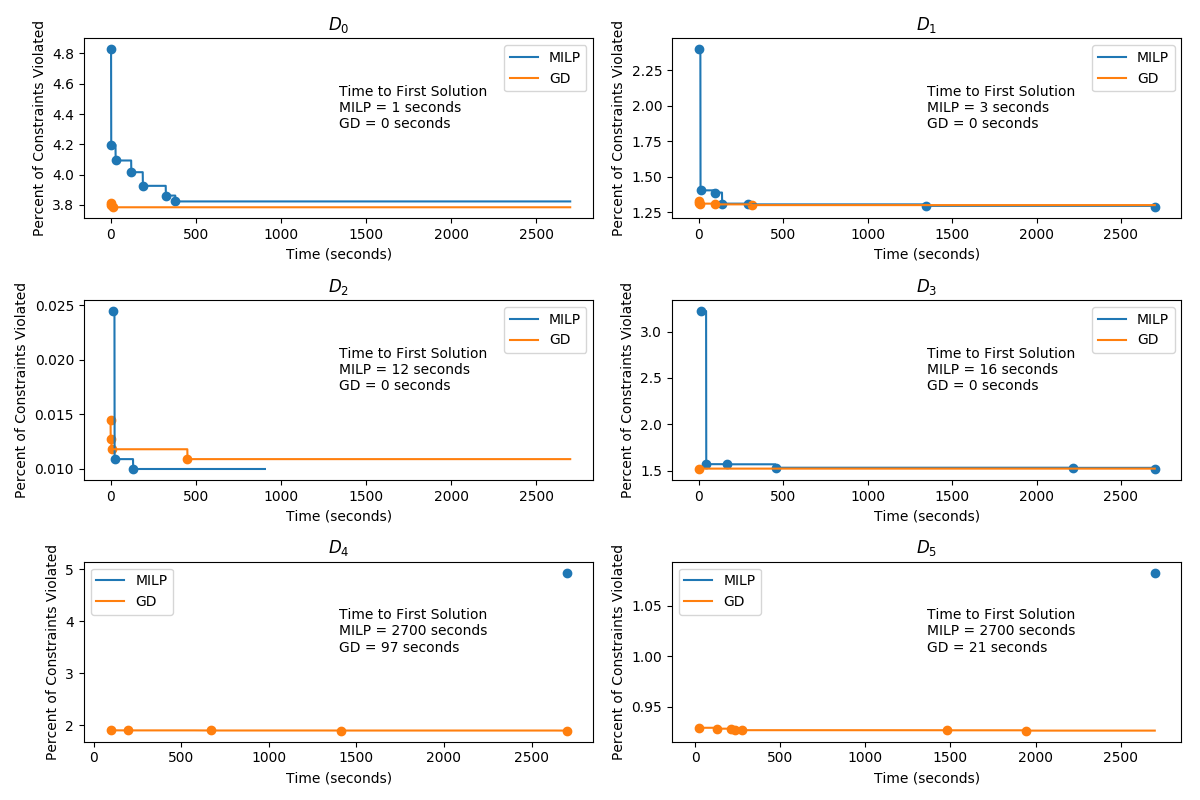
\includegraphics[width=\textwidth]{./time_series.png}
\end{figure}

\section{Discussion}

In this section we discuss the two major takeaways from the experimental results,
the quality of solutions produced and the scalability of the algorithms.

\subsection{Quality of Solutions}

Much to our surprise, the quality of solutions produced by gradient descent
(GD) were very similar, and in some cases even better, than MILP. We attribute this
to the fact that only a single dataset was solved to optimality in the 
allotted time ($D_2$) with MILP.  In fact, despite having an order of magnitude 
fewer constraints then $D_2$, MILP was unable to produce an optimal solution to $D_0$ 
in 12 hours.  This underlines up a key trade off
between the solutions, namely, quality of solutions vs. runtime predictability.
While MILP will produce an optimal solution given enough time and memory, it is
very hard to predict how long it will take to produce an optimal solution. 
In contrast, there are no guarantees that can be made about GD in terms of
the quality of solutions but its runtime is very predictable, scaling
linearly with the number of constraints times the number of columns. 

\subsection{Scalability}

This brings us to our second major point which is the scalability of the
solutions. Examination of the results for $D_4$ and $D_5$, we can clearly see
that GD has superior scaling properties when compared to MILP in terms of
runtime. On both datasets, MILP timed out on both datasets before even
beginning to refine the solution produced, where GD produced a feasible
solution in less than two minutes.  We attribute this disparity to the vastly
different computational complexity of the two algorithms. GD has linear
complexity in the number of constraints in contrast to MILP which has best case
polynomial complexity in the number of constraints. For small problems this not
an issue, but as the problem size increases MILP quickly becomes impractical
even for approximating the optimal solution. Additionally, in order to make the
comparison fair, we ran both solutions on the CPU, however there is nothing to
prevent GD from being run on a GPU. Leveraging GPU compute has the potential to
greatly decrease the iteration time on larger datasets, which would decrease
the time to produce a feasible solution and likely improve the quality of
results.

\section{Future Work}

We identify multiple directions for future work, which fall into 
two categories, optimization techniques, and problem applications. 

\subsection{Optimization Techniques}

In this paper we have only taken a small look at the possible optimization
techniques that could be applied. The most obvious variation that could experimented with
is stochastic gradient descent. This variation has the potential for two major
benefits. First, it can decrease both runtime and memory requirements
of the solution by no longer requiring the entire dataset be processed
on each gradient update. Second, the stochastic version may be able to find
better solutions as it is much more likely that it could escape worse local
minima, instead of relying mostly on having a good starting point.


\subsection{Problem Applications}

We restricted our problem setting to numerical MAX-CSPs with linear
constraints, however in principle there is no reason why this technique could
not be applied to more complex constraints. In particular, non-convex constraints
(e.g. polynomials of degree greater than 2)
would potentially be solved by applying similar techniques, which current
solvers are not able to handle in any capacity. We believe that it is likely
that modifying the optimization procedure, such as using stochastic gradient
descent, will likely be required to provide good approximations of such
functions.

\section{Conclusion}

In this work we have taken brief look at numerical MAX-CSPs, motivated by a
real world use case for tuning full text search engines with labeled data. We
then proposed an algorithm based on gradient descent and ran preliminary
experiments that show it has some key advantages over the baseline MILP based
solution, especially for large problem instances, where commercial solvers are
too slow to be practical. We believe that our solution shows promise for
finding approximate solutions to problem instances which were not previously
tractable with traditional optimization techniques. Future work should continue
to explore the possible variations of the gradient descent algorithm and
explore applying the technique to related problems. 

\bibliographystyle{abbrvnat}
\bibliography{references}
\end{document}
